% ============================================================================
% 3. Method
% ============================================================================
\section{Method}\label{sec:method}

\subsection{Problem setting and notation}\label{sec:notation}
Let $Q, K, V \in \mathbb{R}^{n \times \dk}$ denote the query, key, and value
matrices for a single attention head over a sequence of $n$ tokens, where
$\dk = d_{\text{model}}/h$ is the per-head dimension. Every variant examined in
this study computes
\begin{equation}\label{eq:generic}
  \operatorname{Attn}_s(Q, K, V) \;=\; \operatorname{softmax}\!\left(
  \frac{QK^{\top}}{s}\right)V,
\end{equation}
parameterised solely by the \emph{scaling factor} $s > 0$: the constant by which
the logits are divided before the softmax. The variants differ only in $s$.

\subsection{Attention scaling variants}\label{sec:variants}
The three primary variants are the standard scaled dot-product attention of
Vaswani et al. \cite{vaswani2017}, the alternative $1/\dk$ divisor that removes
the square root, and the temperature-scaled softmax with $\tau = 2$:
\begin{align}
  \operatorname{Attn}_{\mathrm{std}}(Q,K,V)
      &= \operatorname{softmax}\!\left(\frac{QK^{\top}}{\sqrt{\dk}}\right)V,
      & s_{\mathrm{std}} &= \sqrt{\dk} \approx 5.66, \label{eq:standard}\\
  \operatorname{Attn}_{1/\dk}(Q,K,V)
      &= \operatorname{softmax}\!\left(\frac{QK^{\top}}{\dk}\right)V,
      & s_{1/\dk} &= \dk = 32, \label{eq:dk}\\
  \operatorname{Attn}_{\tau}(Q,K,V)
      &= \operatorname{softmax}\!\left(\frac{QK^{\top}}{\tau\sqrt{\dk}}\right)V,
      & s_{\tau} &= \tau\sqrt{\dk} \approx 11.31 \;\;(\tau{=}2). \label{eq:temp}
\end{align}

All three are parameter-free rescalings of the same logits. They introduce no
additional weights, no additional arithmetic of consequence, and no change to
memory traffic. Two auxiliary ablation arms probe the mechanism
(Section~\ref{sec:ablations}): a \emph{mixed-scale} variant in which two of the
four heads use standard scaling and two use $1/\dk$ scaling, and a
\emph{learning-rate compensation} arm in which the learning rates of the query
and key projections of the $1/\dk$ variant are multiplied by
$\sqrt{\dk} \approx 5.66$ to offset the predicted $1/s$ gradient attenuation.
A temperature sweep $\tau \in \{0.5, 1.0, 1.5, 2.0\}$ additionally probes the
direction of the effect around the standard $\tau = 1$ point.

\subsection{Model architecture}\label{sec:architecture}
The backbone is a compact pre-LN Transformer encoder \cite{xiong2020,ba2016}
whose dataflow is shown in Figure~\ref{fig:arch}. Token embeddings
(vocabulary 18{,}855) and learned positional embeddings (maximum length 128) are
summed and passed through two pre-LN encoder blocks, each computing
$\operatorname{LayerNorm} \to$ multi-head self-attention $\to$ residual add,
followed by $\operatorname{LayerNorm} \to$ feed-forward (GELU) $\to$ residual
add \cite{hendrycks2016}. A final LayerNorm is followed by masked mean pooling
over non-padding positions and a task-dependent head: a linear classifier for
SST-2/IMDB (2 classes), AG News (4 classes), or a weight-tied linear language
modelling head for WikiText-2. Dropout ($p = 0.1$) \cite{srivastava2014} is
applied to the embeddings and to the attention and feed-forward outputs. Query,
key, value, and output projections are bias-free linear maps of width
$d_{\text{model}} = 128$ with four heads ($\dk = 32$), and the feed-forward width
is 256. The scaling factor $s$ enters exactly one line of the forward pass: the
division of the logits $QK^{\top}$ inside each attention head.

\begin{figure}[t]
  \centering
  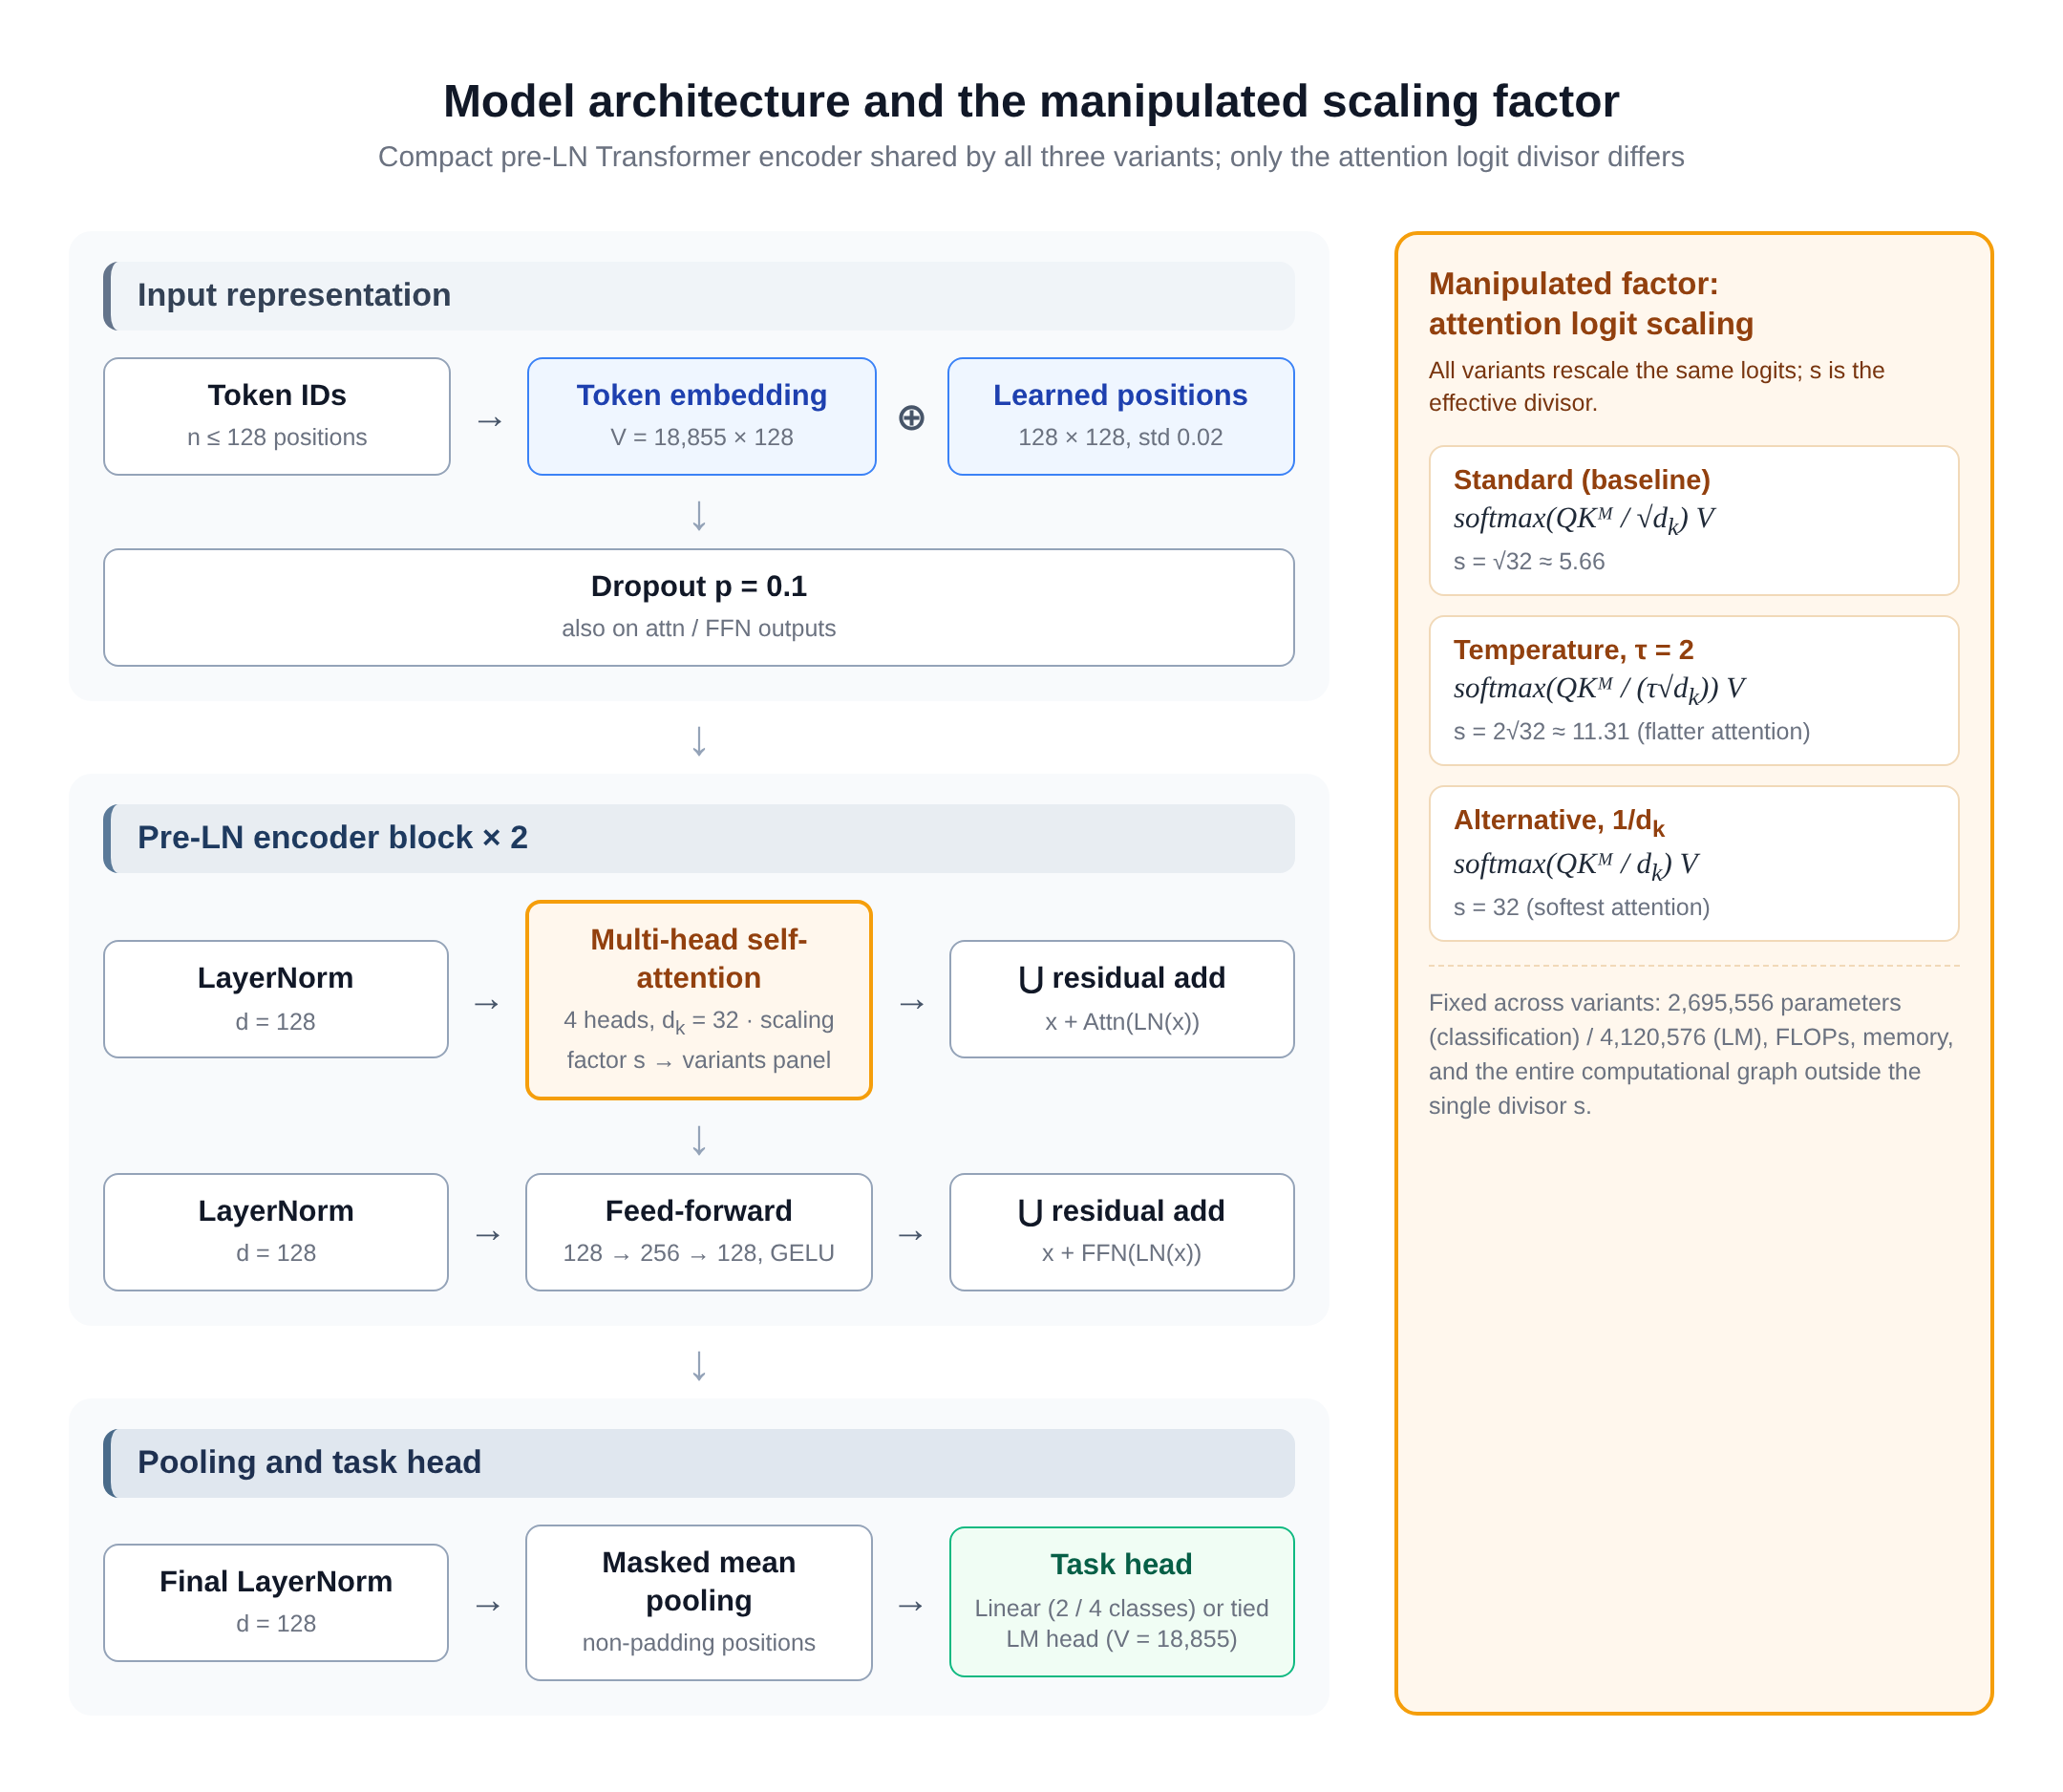
\includegraphics[width=0.94\textwidth]{figures/fig_architecture.png}
  \caption{Model architecture and the manipulated factor. \textbf{Left:} the
  compact pre-LN encoder shared by all variants (2 blocks, 4 heads,
  $\dk = 32$). \textbf{Right:} the three scaling variants, which differ only in
  the effective divisor $s$ of the attention logits. Parameter counts, FLOPs,
  and memory are identical across variants.}
  \label{fig:arch}
\end{figure}

\begin{table}[t]
  \centering
  \caption{Model and optimisation specification (identical for all variants).}
  \label{tab:model}
  \small
  \begin{tabular*}{\textwidth}{@{\extracolsep{\fill}} l l l}
    \toprule
    \textbf{Component} & \textbf{Value} & \textbf{Notes} \\
    \midrule
    Vocabulary / max.\ sequence length & 18{,}855 / 128 & built from training data only \\
    $d_{\text{model}}$ / heads / $\dk$ & 128 / 4 / 32 & per-head dimension \\
    Encoder layers / FFN width & 2 / 256 & pre-LN residual ordering \\
    Projections $W_q, W_k, W_v, W_o$ & $128 \times 128$, bias-free & per block \\
    Activation / dropout & GELU / $p = 0.1$ & \cite{hendrycks2016,srivastava2014} \\
    Pooling & masked mean & non-padding positions \\
    Task head & Linear (2/4 classes) or tied LM head & WikiText-2: weight-tied \\
    Attention logit clamp & $[-50, 50]$ & numerical stability \\
    Parameter count & 2{,}695{,}556 (cls) / 4{,}120{,}576 (LM) & identical across variants \\
    \midrule
    Optimiser & AdamW \cite{loshchilov2019} & $\beta = (0.9, 0.999)$, $\epsilon = 10^{-8}$ \\
    Learning rate / weight decay & $3 \times 10^{-4}$ / 0.01 & \cite{kingma2015} \\
    LR schedule & linear warmup (5\% of steps), cosine decay & \\
    Batch size & 64 (classification) / 16 (LM) & eval.\ 64 / 32 \\
    Gradient clipping & $\max\|g\|_2 = 1.0$ & \\
    Precision & FP32 (mixed precision disabled) & reproducibility \\
    Budgets & 2 epochs (core) / 25 epochs (extended) / 25{,}000 steps (LM) & frozen per grid \\
    \bottomrule
  \end{tabular*}
\end{table}

\subsection{Datasets and preprocessing}\label{sec:datasets}
Four datasets span two task families (Table~\ref{tab:datasets}): topic
classification (AG News, 4 classes \cite{zhang2015}), sentiment classification
(SST-2 \cite{socher2013} and IMDB \cite{maas2011}), and language modelling
(WikiText-2 \cite{merity2017}). All datasets are loaded through the HuggingFace
\texttt{datasets} ecosystem \cite{wolf2020} with fixed splits: classification
training sets are subsampled to 10{,}000 examples with a 20\% held-out
validation split (SST-2 uses the official GLUE validation and test splits), and
WikiText-2 is tokenised into 128-token sequences. Classification text is
tokenised with a lowercased regular-expression pattern (\texttt{[a-z0-9']+});
language modelling uses whitespace tokenisation with an end-of-sequence token.
Vocabularies (top 18{,}855 tokens at minimum frequency 2) are built from
training data only, so no test information leaks into preprocessing. Sequences
are right-padded to length 128 with attention masks that exclude padding
positions.

\begin{table}[t]
  \centering
  \caption{Datasets and splits. Classification training sets are subsampled to
  10{,}000 examples; validation splits follow the repository configuration.}
  \label{tab:datasets}
  \small
  \begin{tabular*}{\textwidth}{@{\extracolsep{\fill}} l l l r r r l}
    \toprule
    \textbf{Dataset} & \textbf{Task} & \textbf{Classes} & \textbf{Train} &
    \textbf{Val} & \textbf{Test} & \textbf{Source} \\
    \midrule
    AG News    & topic classification & 4 & 10{,}000 & 2{,}000 & 7{,}600  & \cite{zhang2015} \\
    SST-2      & sentiment classification & 2 & 10{,}000 & 1{,}115 & 1{,}821 & \cite{socher2013} \\
    IMDB       & sentiment classification & 2 & 10{,}000 & 2{,}000 & 25{,}000 & \cite{maas2011} \\
    WikiText-2 & language modelling &~--- & 36{,}718 seq & 3{,}760 seq & 4{,}358 seq & \cite{merity2017} \\
    \bottomrule
  \end{tabular*}
\end{table}

\subsection{Matched-seed paired design}\label{sec:design}
The core classification grid is 3 variants $\times$ 25 seeds $\times$ 3 datasets
$= 225$ runs at GPU scale; the language-modelling grid (3 variants $\times$
25 seeds) is completed in Stage 2 at replica scale with the corrected causal
mask (Section~\ref{sec:replica-protocol}). Within a seed $s \in \{1001, \dots,
1025\}$, the three variants share (i) a bit-identical parameter initialization
$\theta_0(s)$~--- verified by unit tests that compare initial-state hashes
across variants, (ii) the same training-example order driven by a seeded
permutation generator, (iii) the same optimizer state trajectory shape, and
(iv) the same frozen budget (Figure~\ref{fig:design}). The unit of statistical
analysis is therefore the within-seed difference $d(s) = a_{\text{std}}(s) -
a_v(s)$, giving $n = 25$ paired observations per comparison. This design removes
initialization and data-order variance~--- typically the dominant variance
components in small-model training \cite{bouthillier2021}~--- from the
comparison, and it is exactly the matched-pair structure recommended for NLP
evaluation \cite{dror2018}.

\begin{figure}[t]
  \centering
  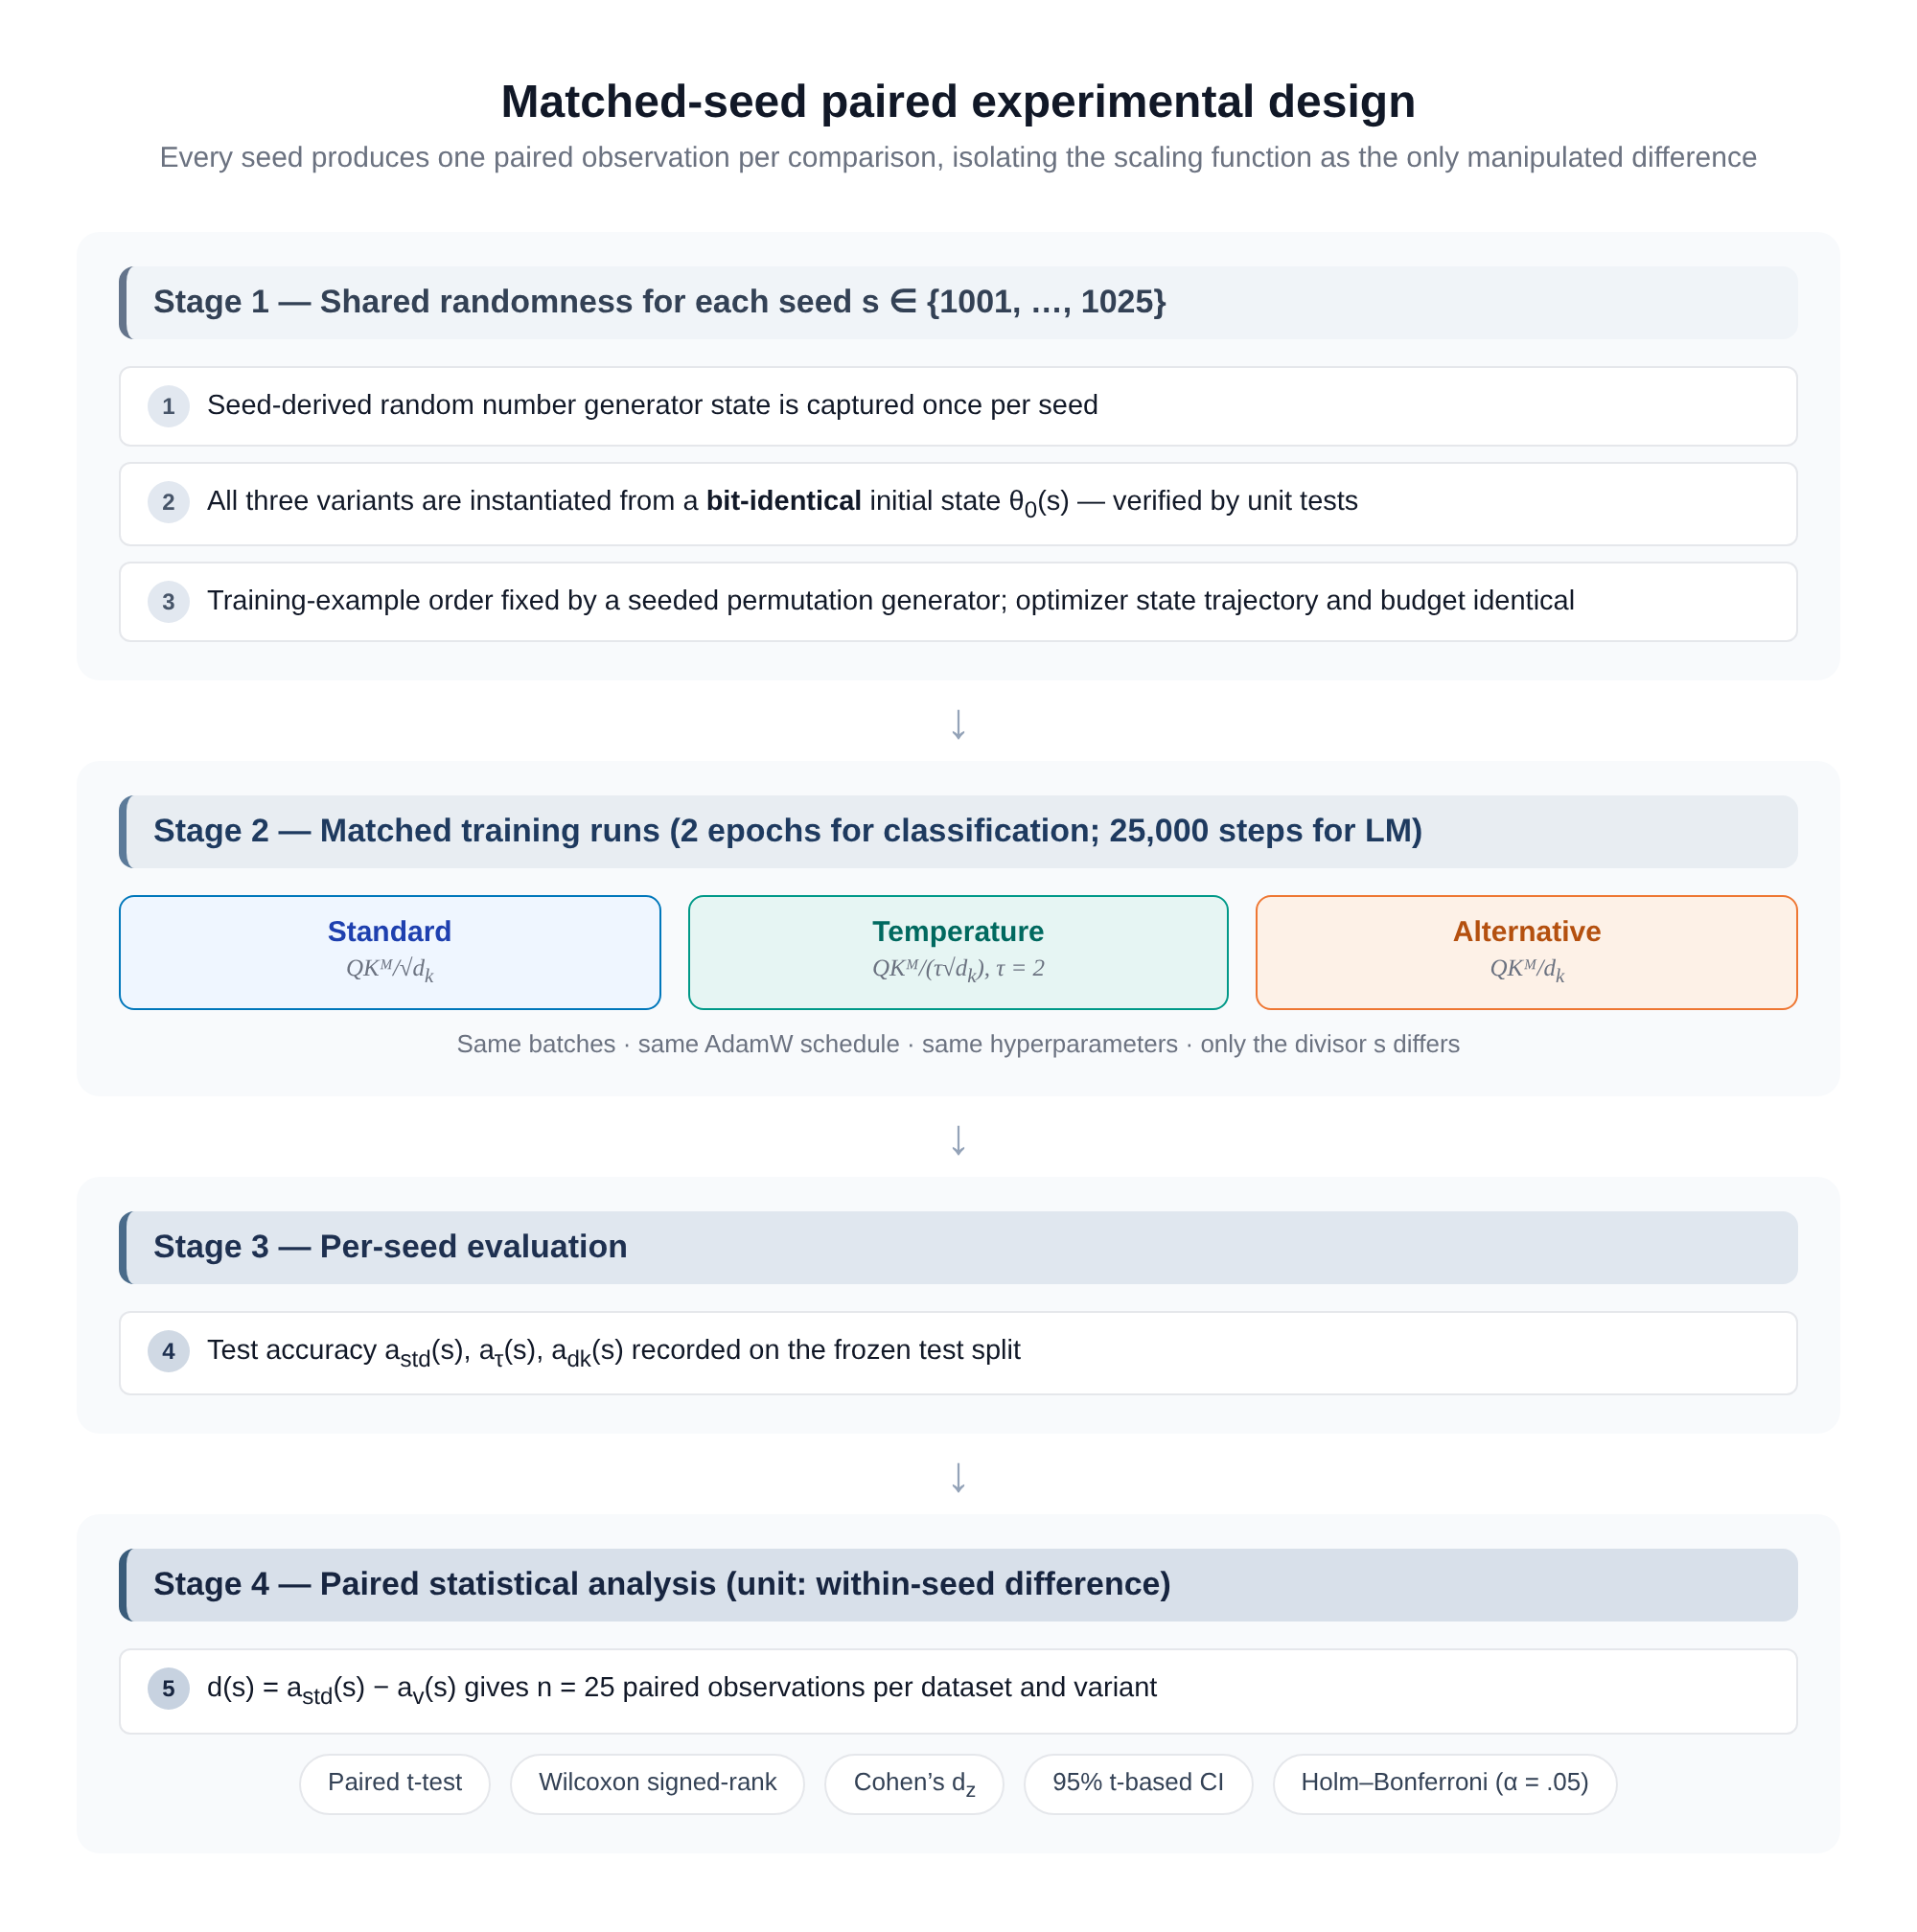
\includegraphics[width=0.9\textwidth]{figures/fig_design.png}
  \caption{Matched-seed paired experimental design. Each seed contributes one
  paired observation per comparison, so the scaling function is the only
  manipulated difference between arms.}
  \label{fig:design}
\end{figure}

\subsection{Stage-2 replica protocol and artifact probes}\label{sec:replica-protocol}
Stage 2 completes the grids that Stage 1 left open on a documented replica
protocol, chosen to fit a 2-core CPU sandbox (3\,GB RAM, PyTorch 2.15 CPU
build) while preserving every structural property of the design: the same
pre-LN architecture, the same three scaling variants with the same effective
divisors, the same matched-seed construction (bit-identical initial state,
shared data order), the same optimizer (AdamW, $\mathrm{lr}=3\times10^{-4}$,
weight decay 0.01, 5\% linear warmup then cosine decay, gradient clip 1.0),
and the same analysis pipeline. The reductions are: 2{,}000-example training
subsets (val 500; test sets 4{,}000/872/2{,}500 for AG News/SST-2/IMDB),
64-token sequences, batch 32, and per-dataset word-level vocabularies built on
the training subset (AG News 7{,}234; SST-2 2{,}249; IMDB 12{,}000; WikiText-2
5{,}655 with 96{,}000 training tokens and 40{,}000 validation tokens). The
replica LM uses $d_{\text{model}}{=}96$, 3 heads ($d_k{=}32$), 2 layers,
$d_{\text{ff}}{=}192$, batch 32, 3 epochs; the classification replica keeps the
original $d_{\text{model}}{=}128$, 4 heads. Seed allocation is 1001--1025 for
the replica core and LM, 1001--1012 for the $\dk$ grid, 1001--1005 for
train-to-convergence, and 1001--1003 for the ablations. Every run is recorded
as an append-only JSONL record keyed by (phase, dataset, variant, $\dk$, seed),
making the grid resume-safe and auditable; 312 pre-registered runs completed
without gaps, plus 27 mask-artifact probes (Section~\ref{sec:lm}).

\subsection{Stage-3 operating-point protocol}\label{sec:stage3-protocol}
Stage 3 manipulates the softmax operating point directly. All arms reuse the
replica architecture, matched-seed construction, and JSONL record protocol of
Section~\ref{sec:replica-protocol}; the new mechanisms are four.
\emph{(i) Divisor power law.} For i.i.d.\ $N(0, \sigma^2)$ logits over $n$
attended positions, the KL divergence between the attention distributions
induced by two divisors is derived to second order in $(b\,\sigma)$
($b = 1/c$; Appendix S17 of the supplementary material) and validated by Monte Carlo
(200{,}000 replicates per grid point; $\dk \in \{32, 128\}$,
$n \in \{64, 128\}$, $\sigma \in [0.5, 16]$).
\emph{(ii) Logit gain.} A scalar $g$ multiplies $q$ and $k$ each by
$\sqrt{g}$ after the output projections and before QK-Norm, so the raw logit
variance scales by $g$ while everything else (initialization, data order,
optimizer trajectory shape) is held fixed; the gain sweep uses
$g \in \{1, 2, 4, 8, 16, 32\}$, 4 seeds, 3 variants (72 runs). The
regime-restored arms train 6{,}000-example AG News for 8 epochs with per-epoch
operating-point probes at $\dk \in \{32, 128\}$ (18 runs), and the LM gain arm
trains the replica LM at sequence length 128 with $g \in \{1, 4\}$
(18 runs).
\emph{(iii) Operating-point probe.} Every Stage-3 run records, per layer, the
raw pre-division logit SD $\sigma_{\text{raw}}$, the realised attention
entropy and maximum weight under the model's own divisor, and the KL
divergence between the attention maps the \emph{same} logits would induce
under each of the three divisors~--- the exact quantity
Eq.~\eqref{eq:law} predicts.
\emph{(iv) Frontier stabilisers and pretrained decoders.} The bridge arms add
per-head QK-normalisation (LayerNorm on $q, k$; affine defaults preserve
bit-identical matched initialization) and Gemma-2-style attention logit
soft-capping ($z \mapsto c \tanh(z/c)$, $c = 3.0$) at gain 32 (20 runs). The
frontier probe loads pretrained GPT-2 checkpoints (124M, 355M) with eager
attention, replaces only the attention scaling factor
($1/\sqrt{d_k} \to 1/d_k$ or $1/(2\sqrt{d_k})$; $d_k = 64$), and evaluates
WikiText-2 validation perplexity over 160 non-overlapping 128-token windows
with per-layer $\sigma_{\text{raw}}$, entropy, and KL diagnostics (6
evaluations). A companion GPU script extends the identical intervention and
diagnostics to 1B--7B HuggingFace decoders (GPT-2-XL, Pythia, Llama-3.2,
Qwen2.5) and is shipped with the repository
(\texttt{scripts/frontier/frontier\_gpu\_1b7b.py}).

\subsection{Statistical analysis}\label{sec:stats}
For each dataset and variant $v$ we compute the paired differences
$d_i = a_{\text{std}}(s_i) - a_{v}(s_i)$, $i = 1, \dots, n$, and report the mean
difference, the 95\% $t$-based confidence interval
\begin{equation}\label{eq:ci}
  \bar d \;\pm\; t_{0.975,\,n-1} \cdot \frac{\operatorname{SD}(d)}{\sqrt{n}},
\end{equation}
Cohen's $d_z$ for paired designs,
\begin{equation}\label{eq:dz}
  d_z \;=\; \frac{\bar d}{\operatorname{SD}(d)},
\end{equation}
with conventional magnitude labels (negligible $|d_z| < 0.2$, small, medium,
large) \cite{cohen1988}, the two-sided paired $t$-test, and the Wilcoxon
signed-rank test as a non-parametric confirmation \cite{wilcoxon1945}. Because
each dataset contributes two comparisons against the common baseline, family-wise
error is controlled with the Holm--Bonferroni step-down procedure
\cite{holm1979} within each dataset at $\alpha = 0.05$. Effect sizes and
confidence intervals are interpreted with the usual cautions for small samples.

\subsection{Implementation, validation, and reproducibility}\label{sec:impl}
The study is implemented in PyTorch with configuration-driven experiment scripts
(YAML), a preflight validator that checks the environment and configurations
before launch, and 22 unit tests in 5 suites covering: bit-identical
initialization across variants for a fixed seed, gradient flow through all
variants, output shapes, masked attention correctness, and data-pipeline
determinism. Mixed precision is disabled and logits are clamped to $[-50, 50]$
for numerical stability. Every run writes a per-seed JSON record (configuration
hash, training history, and test metrics) from which the aggregate tables and
figures in this paper are generated by committed analysis scripts. The full
package~--- source, configurations, tests, per-seed records, statistical
analysis outputs, figures, and this manuscript~--- is released under an MIT
licence.\footnote{\url{https://github.com/razahasan2000/Attention-Scaling}}
